\chapter{Methods} \label{chapter:MD}

\lettrine{M}{olecular Dynamics} simulations have been rightly defined as the `Computational Microscope' \cite{Lee2009,Dror2012} as they offer otherwise inaccessible insights into the molecular details underlying conformational changes of proteins and nucleic acids. Computational methods and tools based on MD are routinely applied in structural biology to quantitatively characterise the dynamics and thermodynamics of proteins and their complexes. The increasing computational power available, and the flexibility of the algorithms which can be implemented on different platforms, have made possible to access molecular dynamical properties inaccessible to experiments. These techniques and the associated force fields are also commonly used in the process of structure determination from NMR data and theoretical structure prediction \cite{Vogel2017,Heo2018}.
%
Modelling and simulating a biological system consists in describing its components and their mutual interactions, and implementing the laws of physics to reproduce its natural evolution. A quantum mechanic description would be more accurate but expensive to achieve for large systems. To facilitate the task, several simplified models have been devised, each most suitable to investigate particular cases.
%
In particular, a large class of models focuses on a classical mechanics description of the dynamics: for increasing sizes of the systems and longer time spans described, the classical approximations will be increasingly accurate, and also the only possible representation computationally affordable.

We briefly present here the core theory and implementation of classical MD simulations, together with a discussion of their strengths, limitations and comparison with experiments. Understanding their methodology provides the interpretative key with which simulations must be designed, run and interpreted in each specific case \cite{vanGunsteren2006}. A review of relevant examples will complete the chapter.


\section{Algorithms for Molecular Dynamics}

\hl{In this section, the core algorithm behind MD simulations is presented, together with the corrections and refinements implemented on it, as it sets the ground for the approximations to follow: as much accurately the system can be modelled, in a classical MD framework it will always be processed by an engine based on classical mechanics rules and finite steps approximations, which inevitable influences the outcome.}

\subsection{The Newton's law}

In a classical MD framework, Newton's second law of motion rules the dynamics, stating that the acceleration $\textbf{a}$ that a particle is subject to at time $t$, depends on the total force $\textbf{F}$ acting on the particle itself and on its mass $m$ (bold denotes vectorial quantities):
\begin{equation} \label{eq:newton}
\textbf{F}(t) =  m \cdot \textbf{a}(t) \, .
\end{equation}
As the acceleration $\textbf{a}(t)$ is the second derivative of the position $\textbf{r}(t)$ with respect to time, given the initial position and velocity of the particle ($\textbf{r}(t_0)$, $\textbf{v}(t_0)$), their temporal evolution can be computed integrating $\textbf{a}(t) = \textbf{F}(t)/m$ as follow:
\begin{eqnarray} \label{eq:analytical}
\mathbf{v}(t) &=& \mathbf{v}(t_0) + \int_{t_0}^t \frac{\mathbf{F}(t')}{m} \, dt' \, ; \\
\mathbf{r}(t) &=& \mathbf{r}(t_0) + \int_{t_0}^t \mathbf{v}(t') \, dt' + \int_{t_0}^t \int_{t_0}^{t'} \frac{\mathbf{F}(t')}{m} \, dt'' \, dt'\, . \label{eq:analytical2}
\end{eqnarray}
%
In the case of complex biomolecular systems with many particles and multiple interactions acting between them, it is impossible to integrate analytically Equations \ref{eq:analytical}-\ref{eq:analytical2}, while a different and feasible approach consists in discretising the equation of motion \ref{eq:newton}.
%
The idea is to consider very short time steps of length $\Delta t$, so that in such intervals the forces are (almost) constant, and the integration of Equations \ref{eq:analytical}-\ref{eq:analytical2} becomes trivial.
%
\hl{The simplest choice consists in considering for the integration both the acceleration and the velocity at time $t_0$, producing the Euler algorithm:}
\begin{eqnarray} \label{eq:euler}
\mathbf{v}(t_0 + \Delta t) &=& \mathbf{v}(t_0) + \frac{\mathbf{F}(t)}{m} \, \Delta t \,; \\
\mathbf{r}(t_0 + \Delta t) &=& \mathbf{r}(t_0) + \mathbf{v}(t_0) \, \Delta t + \frac{\mathbf{F}(t)}{m} \, \Delta t^2 \,. \label{eq:euler2}
\end{eqnarray}
%
\hl{This procedure contains approximation of the order of $(\Delta t)^2$ that will accumulate step after step, biasing greatly the outcome. However, a careful choice of the values to integrate allows to reduce consistently this approximations. For example, choosing the acceleration value at time $t_0$ but the velocity at time $t_0 + \Delta t/2$ decreases the error down to orders of $(\Delta t)^4$. This framework is at the basis of the so-called leap-frog algorithm, which is used in the vast majority of MD engines:}
\begin{eqnarray}
\mathbf{v}\left(t_0 + \frac{\Delta t}{2}\right) &=& \mathbf{v}\left(t - \frac{\Delta t}{2}\right) + \frac{\mathbf{F}(t)}{m} \, \Delta t \, ; \\
\mathbf{r}(t_0 + \Delta t) &=& \mathbf{r}(t_0) + \mathbf{v}\left(t_0 + \frac{\Delta t}{2}\right) \, \Delta t \, .
\end{eqnarray}
This algorithm can thus ``solve" every possible Newton equation, at the expenses of some precision.

\hl{Considering that MD deals with bonded atoms belonging to multi-atoms molecules, the length of these bonds must be kept within a physically meaningful value. Despite the forces acting between single atoms tend to maintain them in the correct geometry, the approximate procedure mentioned above may give raise to unphysical configurations. To correct this, constraint algorithms are applied after the update of atoms positions. The ones used in this work are LINCS (Linear Constraint Solver) \cite{Hess1997} and SETTLE \cite{Miyamoto1992}: the first finds a solution iteratively within an approximation tolerance, as the problem of constraints is hardly solvable analytically; the second is an exact implementation of the solution for rigid bodies of three elements only, and as such is useful for the treatment of water molecules (which have three atoms in their atomistic description).}

\subsection{Thermostats and barostats}
\hl{As an addition to the constraints algorithms mentioned above, other specific algorithms have been developed to more realistically reproduce the simulation's conditions of choice, for example Temperature and Pressure.}

Most experiments are conducted under constant temperature, so that it is desirable to reproduce this condition in simulations.
%
To set up a temperature, at the beginning of the simulations particles can be given random initial velocities distributed according to the Maxwell-Boltzmann curve, which describe velocities of atoms of a noble gas at temperature $T$. The velocity of each of them will be influenced by the specific interactions occurring in the system but, in a constant temperature environment, the total average kinetic energy (proportional to $T$) must remain constant.
%
Even in absence of any dissipative term in the dynamics, the approximations performed in the MD algorithm make this quantity to drift away from its initial value, therefore to ensure temperature is maintained throughout the simulation, thermostat algorithms have been devised.

The principle behind a thermostat consists in rescaling the velocity of one or few selected particles at fixed interval of times, to restore the correct average kinetic energy. This fixed interval of time must not correspond to the timestep itself, as the goal of a thermostat is to maintain the average temperature, and not its value at all times, as fluctuations are allowed in natural systems.
%
Moreover, it is strongly recommended to couple solute and solvent to separate baths, to ensure that both maintain the correct temperature. Indeed, it is possible that the energy exchanged between solute and water (or other components) is not perfect, due to different conditions adopted for their simulations, like cut-offs or restraints.
%
The most used thermostat algorithms are the Berendsen \cite{Berendsen1984}, Nos\'{e}-Hoover \cite{Nose1983,Hoover1985}, Andersen \cite{Andersen1980} and velocity rescale \cite{Bussi2007}, which differ in the quantities selected for such rescaling.

Another macroscopic condition one wish to maintain is either the volume or the pressure of the system. While maintaining the volume constant is easy (and, combined with constant temperature, gives the NVT ensemble), pressure regulation (i.e. maintaining a NPT ensemble) requires a barostat.
%
Pressure is directly proportional to the average quantity of motion exchanged between the particles and the walls of the box they are confined to, which depends on the frequency of collision and thus on the extent of the box. Barostats change the box size to regulate the pressure.
%
It has to be noticed that most MD simulations are run under periodic boundary conditions, i.e. a particle which exits from the simulation box during a move is brought back on the opposite side of the box, leaving the box density constant. This mimics the presence of an infinite number of equivalent boxes one next to the other, and alleviates the finite size effects that arise when simulating small systems.
%
In this scenario, particles are not bouncing on the box walls, rather a virtual pressure is computed from the velocities of the ones trespassing the box boundaries during a move.
%
Similarly as for thermostats, the coupling frequency of barostats must be larger than the time step. Usually all the box dimensions are rescaled by the same amount. However, in the case of anisotropic systems like lipids, to maintain the correct pressure, the directions parallel to the membrane plane can be rescaled separately with respect to the one perpendicular to it.
%
Also for pressure coupling several algorithms can be used: the Berendsen \cite{Berendsen1984}, Parrinello-Rahman \cite{Parrinello1981}, or Martyna-Tuckerman-Tobias-Klein (MTTK) \cite{Martyna1996} (to be used in conjunction with the Nos\'{e}-Hoover thermostat), which differ in the way they approach the desired pressure (e.g. exponentially, in an oscillatory way, etc.).


\section{The force field problem} \label{sec:ff}

Once the equations of motion and the control algorithms are set up, the next challenge is represented by modelling the forces and thus the potential energy function.
%
Force fields for classical MD simulations usually rely on the breakdown of interactions into several, independent terms, identified on an empirical physical basis. We report here the functional form adopted for the GROMOS force field \cite{Oostenbrink2004,Schmid2011} as implemented in the GROMACS MD engine \cite{Berendsen1995,Abraham2015,gromacs_man}, as an example of the structure of a classical force field.
%
Other force fields can have slightly different implementations, however, the general classification of interactions and the type of functional forms used are similar.

\paragraph{\hl{Covalent (bonded) interactions}} Covalent interactions are modelled with potential energy terms representing bond stretching, angle bending, improper and proper dihedral angles torsion.
%
The functional form of the potential-energy for bonded interactions aims at a simplified, semi-classical description of the sub atomic motion of molecules, assuming harmonic-like vibrations around the equilibrium position of the bond, angle or dihedral in exam.

Specifically, in the GROMOS force field, a bond between atoms $i$ and $j$ is described by a fourth power potential (similar to a harmonic form, but computationally more efficient):
\begin{eqnarray}
&& V_b(\textbf{r}_{ij}) = \frac{1}{4}\,k^b_{ij}\,\left(|\textbf{r}_{ij}|^2 - b_{ij}^2\right)^2
\end{eqnarray}
where the force constant $k^b_{ij}$ is given in kJ/mol/m$^2$ and $b_{ij}$ is the equilibrium position of the bond between atom $i$ and $j$.

The deviation of the angle between three atoms $i$, $j$ and $k$ from the preferred value $\theta^{\, 0}_{ijk}$ are implemented through a cosine based angle potential:
\begin{eqnarray}
&& V_a(\theta_{ijk}) = \frac{1}{2}\,k^\theta_{ijk}\,\left(\cos\left(\theta_{ijk}\right) - cos\left(\theta^{\, 0}_{ijk}\right)\right)^2 \\
&& \text{with:} \ \cos\left(\theta_{ijk}\right) = \frac{\textbf{r}_{ij}\cdot \textbf{r}_{kj}}{r_{ij}\,r_{kj}}
\end{eqnarray}
with $k^\theta_{ijk}$ in kJ/mol.

Improper dihedrals are used to ensure ring planarity and control the chirality of some tetrahedral centres. They are described through a harmonic potential:
\begin{eqnarray}
&& V_{id} (\xi_{ijkl}) = \frac{1}{2}\,k_{ijkl}^\xi \left( \xi_{ijkl} - \xi_{ijkl}^{\, 0} \right)^2
\end{eqnarray}
where the $\xi$ values are given in degrees and the force constant in kJ/mol/rad$^2$. By convention, the improper dihedral for a set of four atoms $i$, $j$, $k$ and $l$, is taken as the angle between the plane defined by atoms ($i$, $j$, $k$) and the one defined by atoms ($j$, $k$, $l$).

Finally, the last bonded interaction is represented by proper dihedrals, described though a periodic potential:
\begin{eqnarray}
&& V_d(\phi_{ijkl}) = k_{ijkl}^\phi\,\left( 1 + \cos\left( n \, \phi_{ijkl} - \phi_{ijkl}^{\, 0} \right) \right)
\end{eqnarray}
following the convention that $\phi_{ijkl}$ is the angle between the ($i$, $j$, $k$) and ($j$, $k$, $l$) planes, with $i$, $j$, $k$, and $l$ four subsequent atoms (for example along a protein backbone). A value of zero for a proper dihedral corresponds to a \textit{cis} configuration; $n$ denotes the number of equally spaced minima available for the dihedral in a 360$^\circ$ turn. The constant $k_{ijkl}^\phi$ is expressed in kJ/mol.

It must be noticed that these potentials can not model the rupture of a bond: for this, more sophisticated descriptions are needed.


\paragraph{Non bonded interactions}
Non bonded interactions include the short range Pauli repulsion, the ``mid"-range van der Waals attraction, and the long range electrostatic term.

The first two can be modelled together by a Lennard-Jones potential. Its functional form, describing the interaction between two neutral atoms at distance $r$, models the long range dispersion with a $r^6$ behaviour typical of the dipole-dipole interactions found in noble gases (London dispersion forces), while the Pauli term is represented by a $r^{12}$ behaviour to ease the computation in relation with the previous one:
\begin{equation}
V_{LJ}(r) = 4 \epsilon \left[ \left( \frac{\sigma}{r} \right)^{12} - \left( \frac{\sigma}{r} \right)^6 \right].
\end{equation}
Two parameters, $\epsilon$ and $\sigma$, tune the interaction strength and the equilibrium distance. They are fitted against experimental data and are specific of each pair of atoms species.

The Coulomb energy between two charges $q_1$ and $q_2$ at distance $r$ is represented by the Coulomb law:
\begin{equation}
V_C(r) = \frac{1}{4 \pi \epsilon_0} \, \frac{q_i q_j}{\epsilon_r r_{ij}}
\end{equation}
with $\epsilon_0$ the dielectric constant of vacuum and $\epsilon_r$ the relative dielectric constant, introduced to properly take into account the screening provided by the material surrounding the object, as polarisability is not included in this description.

\hl{The treatment of non-bonded interactions requires particular care because of their long range nature: in every point of the simulation box many forces from distant atoms are acting at the same time, making the prediction of the outcome difficult and small shift in the parameters choice can give very different ``macroscopic" results.
%
The van der Waals forces decay fast, therefore the tail of their functional can be cut after a threshold distance with little impact on the outcome; while Coulomb interactions, with their slower decay, must be taken into account throughout the whole simulation box. Many algorithms have been devised to efficiently compute them, like the Particle Mesh Ewald \cite{Essmann1995} or the Reaction Field \cite{Tironi1995} approaches.}

Finally, all biomolecular force fields, and in particular their van der Waals interactions, are parametrised to describe systems at room temperature, therefore simulations performed at substantially different temperatures must be interpreted carefully.


\subsection{Force fields: classifications} \label{sec:ff_ex}

\begin{figure}[p!]
\centering
\includegraphics[scale=.65]{2methods/pics/picture_chapter}
%
\caption[MD force field classifications]{List of most popular simulation force field for biomolecules, ordered from detailed to coarse (reference to the relative papers in Section \ref{sec:ff_ex}). On the left, snapshot of notable systems simulated with the force fields CHARMM (adapted with permission from \cite{Lipkin2017}. Copyright (2017) American Chemical Society); GROMOS (adapted with permission from \cite{Macpherson2019}); SIRAH (adapted with permission from \cite{Machado2017}. Copyright (2017) American Chemical Society) and MARTINI (adapted with permission from \cite{Samsudin2017}). Copyright (2017) Elsevier).}
\label{fig:ff}
\end{figure}

Many force fields for classical MD simulations adopt a functional form equal or similar to the one described above. Their difference lies in the number of degrees of freedom modelled, in a hierarchy of descriptions proceeding from detailed to coarse (Figure \ref{fig:ff}). Three possible classes of descriptions are:
\begin{itemize}
\item all-atoms force fields, where all the atoms are presented in the description, and represented as spheres of variable size according to their van der Waals radius (e.g.\ proportional to $\sigma$ in a Lennard-Jones model). Examples of all-atoms force fields are AMBER \cite{Maier2015,Dickson2014,Wang2004_amber}, CHARMM \cite{MacKerell1998,Klauda2010,Huang2013} and OPLS all-atom \cite{Jorgensen1988}.
\item united atoms force fields, similar to the previous ones but where non-polar hydrogens are incorporated in the heavy atom they are bonded to. The ``united atom" is given a new $\sigma$ parameter and increased mass according to how many hydrogen it includes. The GROMOS force field \cite{Oostenbrink2004,Schmid2011} follows this philosophy. The OPLS force field has also a united atom version \cite{Jorgensen1996}.
\item coarse-grain force fields, which group together in one unique bead few atoms, to reduce the number of variables to compute. The clustered atoms are such that their mutual distances are expected to vary little with respect to the ample movements of components of the system far away from each other (which will be grouped in different beads). The MARTINI \cite{Marrink2007,Monticelli2008,DeJong2013} and SIRAH \cite{Machado2018,Barrera2019} force fields belong to this category.
\end{itemize}
%
We now give a more detailed insight in the characteristics and parametrisation strategies of the atomistic and coarse-grain force fields which will be employed in the work of this thesis.

\subsection{The GROMOS force field}
\hl{All-atoms and united atoms force field are parametrised against first-principle or experimental values.}
%
While for the all-atom force fields AMBER and CHARMM the parametrisation is based on ab initio quantum mechanics calculations refined against experimental data \cite{Maier2015,Dickson2014,Wang2004_amber,MacKerell1998,Klauda2010}, the united atom GROMOS force field relies on the reproduction of heat of vaporization of small molecules and free enthalpies of solvation of small compounds in different solvents, at physiological temperatures and pressures \cite{Oostenbrink2005,Schmid2011,Reif2013}.
%
This procedure sets not only the constants of the bonded interactions, but also the partial charges of the atoms inside a molecule: as no electrons are included for the sake of efficiency, their redistribution across atoms which are bonded is modelled through fractional charges assigned to each atom (while the total charge of a molecule must sum to an integer).
%
Moreover, it is assumed that the parametrisation performed for small moieties can be transferred to a larger compound including these moieties. This limits the number of chemical groups to be described in order to simulate biomolecules.

In every MD simulation, the description of water is crucial. Out of the many water model proposed, the GROMOS parametrisation has been performed with a flexible simple point charge (SPC \cite{Berendsen1981}) model. This description represents water as a three atoms molecule, with a negative charge on the oxygen and a positive complementary one on the two hydrogen atoms, and allows flexible hydrogen-oxygen bonds. This model reproduces correctly the density and dielectric permittivity of water. \hl{To be noticed that, computationally wise, water molecules are the vast majority of the particles involved in a simulation and thus a significant fraction of the computer time is spent in updating their positions.}

The improvement of computational techniques and reparametrisation strategies prompts the periodical release of newer versions of force fields. \hl{In the present work, we employed version 53a6 of the GROMOS force field \cite{Oostenbrink2004} for the set of simulations involving peptidic assembly in solution, while we switched to 54a8 \cite{Schmid2011} for the simulations involving biological membranes. While it is advisable to always have a coherent set of parameters across simulations, to compare their outcome in a consistent manner, when extending the system simulated to include membranes, we deemed the 54a8 parameter set more suitable because of the improvements introduced in the phosphocholine head parametrisation (see Chapter \ref{chapter:lip_par} for a complete discussion on lipid parametrisation in GROMOS).}


\subsection{\hl{The SIRAH force field}}
Two approaches are possible to develop a coarse-grain description: parameters can be fit directly to global quantities derived from experiments, as performed for GROMOS, in a top-down approach; or coarse-grain simulations results can be fit to the outcomes from atomistic ones, in a bottom-up approach.

The coarse-grain force field SIRAH \cite{Machado2018,Barrera2019} is a top-down force field derived to fit structural properties of proteins. It aims at reducing the complexity of an atomistic description while still being able to reproduce the correct secondary structure of proteins across a wide variety of folds contained in the PDB, together with a correct representation of their dynamics.

To obtain this, it opts for a non-uniform granularity, i.e.\ according to the region of interest a different number of heavy atoms is grouped in a bead, from a minimum of two up to four. Regarding proteins, it maintains the backbone flexibility by grouping NH, C$_\alpha$H and CO in three different beads, while the side chains are represented with less details, generally grouping three atoms together. A schematic of the mapping for each amino acid is shown in Figure \ref{fig:sirah}. Contrary to force fields where the amino acid backbone is mapped to one bead only, the SIRAH description allows to reproduce secondary structures without recurring to additional constraints.
%
The dual granularity approach is based on physico-chemical intuition, and is more difficult to generalise than a uniform one. Never the less, the force field has been recently extended to lipids \cite{Barrera2019}, while it comprised a parametrisation for DNA molecules since its infancy.
%
\begin{figure}[h!]
\centering
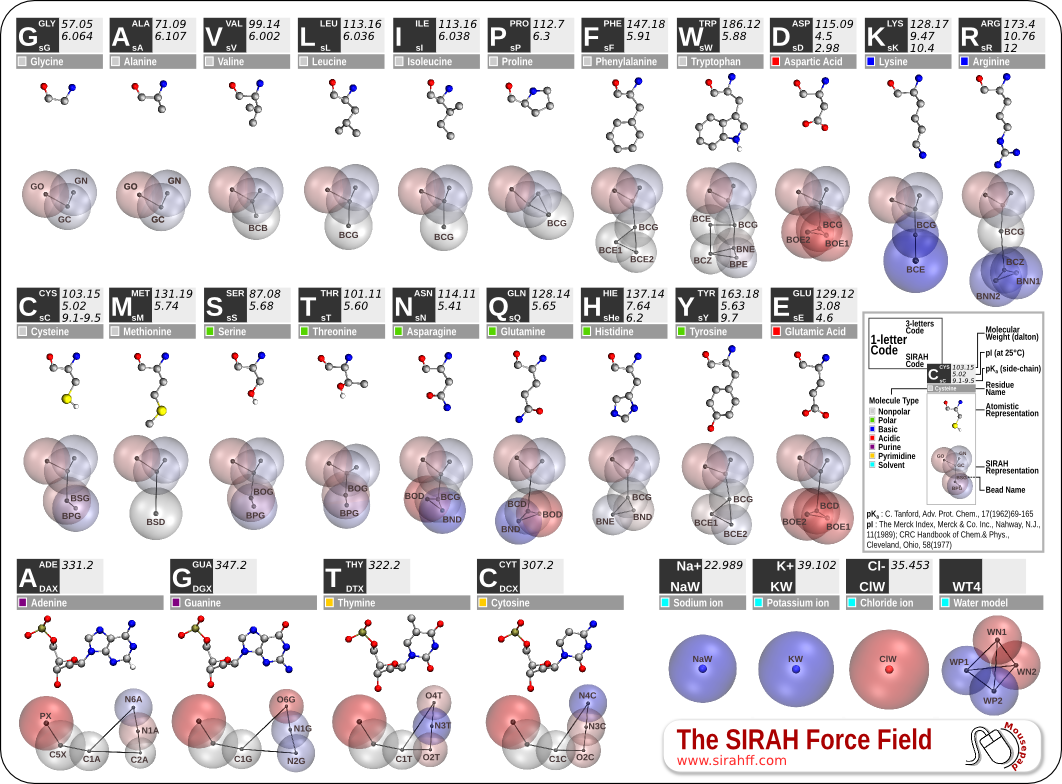
\includegraphics[width=0.8\linewidth]{2methods/pics/sirah_aa.png}
%
\caption[SIRAH force field amino acid and DNA description]{Description of amino acids and nucleic acids in the SIRAH force field.}
\label{fig:sirah}
\end{figure}

The modelling of water in a coarse-grain force field is also critical: usually, a few water molecules are grouped together in one bead. This has two implications: water particles are large and thus cannot solvate very narrow pockets; moreover, collapsing the molecules in one single point in space removes the separation of charges and thus the characteristic dipole every water molecule has. The dipole of water is responsible for hydrogen bonds formation and for the electrostatic screening observed in an aqueous solution. Such screening can be roughly modelled tuning the relative dielectric constant, but as this is a mean field approach, it cannot account for local effects.
%
To partially obviate to that, SIRAH force field maps four waters to a tetrahedral molecule, with one bead on each vertex: all the bonds are rigid, and the structure serves the purpose of having a repartition of plus and minus charges, by assigning a positive charge to two vertices and the opposite charge to the other two, giving a polarisable structure. The geometrical arrangement reproduces the tetrahedral network of water molecules observed in its liquid state, which is characteristic of this fluid and tunes its remarkable properties.

Based on the above premises, SIRAH force field simulations of different peptides and proteins in solution proved to match the relative NMR results, showing a good reproduction of secondary structures; simulations of lipids randomly oriented in water showed the formation of an organised bilayer, and finally the expected behaviour of a few transmembrane proteins in model membranes was correctly reproduced \cite{Machado2018,Barrera2019}.

 
\subsection{The MARTINI force field}
The MARTINI force field is another popular coarse-grain description of biological molecules \cite{Marrink2007,Monticelli2008,DeJong2013}: developed originally with a focus on lipids, much prior to SIRAH, it has been then extended to include proteins, small ligands and DNA/RNA molecules.

MARTINI opts for a four-to-one approach, i.e.\ four heavy atoms are grouped in one bead, resulting in a uniform graining and a coarser description than the SIRAH one. \hl{The only exception to this scheme is represented by rings molecules, where a two-to-one approach is needed to maintain the circular topology (consequently, these beads have a reduced mass with respect to the others, all described with the same mass value).}

The number of bead types has been kept to the minimum necessary to represent biological molecules. They are organised systematically in polar, non-polar, apolar, or charged, and each type has a number of subtypes with increasing polarity to differentiate the chemical nature of the underlying atomistic structures.
%
This systematic parametrisation can be easily transferred to new compounds, without the need of introducing new bead types, analogously to what GROMOS does when parametrising small moieties.

Similarly to GROMOS, the MARTINI force field chooses a top-down approach to parametrise non-bonded interactions, tuning them against experimental partitioning free energies between polar and apolar phases, while bonded interactions are derived from reference all-atom information, in a bottom-up approach.
%
Specifically, they are designed so that the results from coarse-grain simulations match the structural data of the underlying atomistic geometry, derived either from available structures or atomistic simulations. \hl{For example the distribution of the length of a bond in a molecule would be mapped to its coarse-grain version (i.e. computing the corresponding bead-to-bead distance) and compared with the respective one obtained from coarse-grain simulations.}

The four-to-one mapping implies that the amino acid backbone is represented by one bead only, preventing the description of directional bonds which are key to reproduce the secondary structure. The bonded parameters partially account for this, favouring for each residue type the backbone conformation in which it is most likely found (as computed from the Protein Data Bank - PDB \cite{PDB}). When this is not sufficient, the protein can be constrained around a given structure through an elastic network model approach (ElNeDyn \cite{Periole2009}). However, both the backbone parametrisation and the use of ElNeDyn imply that conformational changes in the structure are penalised and therefore not well sampled in MARTINI simulations.

The MARTINI force field provides two water model. The standard one groups four water molecules in one bead only, loosing the polarisability typical of water molecules, the effect of which is partially restored with the use of a high dielectric constant. The polarisable water model \cite{Yesylevskyy2010} maps instead four water molecule to a single ``inflated" water, i.e.\ a three-beads molecule with the same shape of a single molecule, but expanded, and a charge splitting which can account for the water dipole. \hl{This model allows to revert the dielectric constant back to a value closer to 1 (where an exact value of 1 corresponds to no mean-field correction to the electrostatic interactions, meaning they are correctly modelled by the collective action of the atoms/beads described).}

\hl{Overall, the MARTINI force field pushes the limits of simplification to enhance the simulations speed-up, with considerable gain in efficiency with respect to atomistic or even SIRAH simulations. Despite it can not capture some fine details of the systems studied, it has been successfully applied to describe the behaviour of many biological membranes \cite{Khalid2019,Samsudin2017}, lipid self-assembly \cite{Marrink2007} and peptide-membrane binding \cite{Song2019}. The (re)introduction of a more detailed water model allowed the description of electroporation processes and translocation of ions through bilayers \cite{Yesylevskyy2010}.}

\subsection{Backmapping techniques} Coarse-grain descriptions are very effective in reproducing long time scales; however, to retrieve finer details after such extensive exploration, backmapping techniques have been designed to obtain atomistic configurations from the coarse-grain ones \cite{Wassenaar2015}. These backmapped structures can in turn be simulated at the atomistic level to explore the short time scale movements around such interesting conformation. The easy transfer between the two resolution, gave rise to many multiscale studies applied to biomolecular systems \cite{Lee2012}.


\section{Beyond the classical framework}

Without entering into the details, it is important nevertheless to mention that the classical MD framework can benefit on one side of refinements which improves its accuracy, and on the other side of specific techniques which instead speed up the calculations, at the expenses of the loss of some details.

\paragraph{Polarisability and quantum effects}
The first refinement possible is the introduction of polarisability, i.e. the displacement of electrons with respect to the nucleus, as a consequence of the surrounding electrostatic environment. None of the force fields mentioned above accounts for that, because electrons and nucleus of an atom are modelled as a unique object. Specific force fields have been modelled to include this effect, either on top of atomistic descriptions, as in AMOEBA \cite{Ren2003,Ponder2010}, Drude polarisable CHARMM \cite{Anisimov2004} or AMBERff02 \cite{Cieplak2001}, or in combinations with a coarse-grain descriptions, as in the ELBA force field \cite{Orsi2011}. Polarisability does improve the accuracy of simulations (see Chapter \ref{chapter:lip_par}, where it is discussed in the context of lipid tails parametrisation), but it can significantly slow down simulations.
%
Moreover, for biological processes governed by quantum mechanics - such as photosynthesis, DNA mutation processes or some enzymatic activities - many semi-classical hybrid techniques have been developed \cite{Ahmadi2018}. They combine computational quantum mechanical modelling methods, such as Density Functional Theory (DFT) or Hartree-Fock computations (HF) \cite{Shao2015}, with classical Molecular Dynamics to gain the accuracy of a quantum description in the region of interest and the speed up of a classical one in the surrounding areas.

\paragraph{Reduction of the number of degrees of freedom}
\hl{At the other end of the spectrum, tackling instead efficiency issues, many models have been implemented to reduce the number of degrees of freedom to deal with, among which the coarse-grain force fields already mentioned.}
%
Another approach is constituted by implicit solvent, where water is represented as a continuous medium, as opposed to explicit models which include all its particles \cite{Kleinjung2014}.
%
Models of implicit solvent can be based on different assumptions: for example the solute-solvent interactions can be taken as proportional to the solvent accessible surface area (SASA) of every particle of solute \cite{Fraternali1996,Kleinjung2003,Kleinjung2012,Fornili2012}, or instead can be derived from a solution of the Poisson-Boltzmann equation governing the charge density in a material, for example in the form of the Generalised Born equation \cite{Zhu2005} which is valid under particularly simple conditions.
%
Another technique to alleviate the computational burden is constituted by hybrid particle-field algorithms. The idea is to treat non-bonded interactions through a mean field approach, where atoms/beads move in the field generated by the others. The field does not need to be updated at every time step, as it is a collective and thus slowly evolving variable; moreover, for each particle only the interaction with the field, and not with all the neighbour particles needs to be computed, reducing the computations effort further. This approach has been employed with a coarse-grain description of polymers and biological molecules in the OCCAM software \cite{Milano2009}.

\paragraph{Enhanced MD techniques}
Finally, computational strategies have been devised to bias the natural evolution of the system in order to enhance the sampling of many configurations, i.e. to speed up its pace.
%
\hl{This is necessary when the natural evolution of the system exceeds the computational time available. This scenario can correspond to transitions between two states separated by an energy barrier - for example between two favourable conformations of a protein, but matches also a more general question that MD is often call to answer: the exploration of the phase space. Indeed very often, in the impossibility of understanding from first principles which states of a system are the most energetically favoured, and thus can influence its macroscopic behaviour (up to entropy effects), MD simulations are run to explore the broadest possible set of them. This would not only allow to compute the energy for each of them and identify minima, but also provide informations of the entropic contribution through the time spent in each of them.}

\hl{However, the above procedure works only in an ideally infinitely long simulation which has sampled all the possible states. As biomolecular systems have a complex landscape dense of energy barriers, a realistic, limited time simulation usually samples regions around the initial configuration only.
%
In the simulations of proteins, this would often correspond to a structure derived from X-ray crystallography, which might not represent the native state of the protein in solution nor the functional form of interest.
%
For this reason, in the present work, the use of different initial structures would allow the exploration of an otherwise prohibitively large phase space.}

The challenges mentioned above have promoted the development of enhanced MD techniques. As a non comprehensive list, we mention replica-exchange algorithms \cite{Okamoto2004} which combine together multiple simulations held at different conditions, local potential-energy elevation (or metadynamics) \cite{Huber1994,Laio2002} which avoids the re-sampling of already visited conformations adding an energy penalty to them, umbrella sampling \cite{Torrie1977} which reconstructs free-energy barriers from simulations held at specific values of the coordinate along which the barrier exists, or finally simply the use of higher temperature to overcome energy barriers \cite{Kirkpatrick1983}.
%
\hl{To be noticed that a coarse-grain description of a system, by reducing the number of degrees of freedom, discards the high-frequency or less interesting ones, giving a smoother energy surface, so that the search is speed up both by the reduced computational load and by the fact that the system is not trapped into local minima due to the landscape roughness.}


\section{MD and experiments: ensembles versus averages}
The validation of MD simulations is performed by comparison with experiments: the properties obtained experimentally are computed from the MD trajectory as well, and the latter compared with the former. If these are correctly reproduced, it is usually assumed that the simulation is sampling the correct ensemble of states. This holds if the properties of the simulation are not drifting away, namely the system has reached equilibration and it is thus in a stationary state.
%
Once the simulation has been validated, one can identify, from the conformations in the trajectory, the details of the processes responsible for the experimental outcome of interest, as such information is not accessible by the experiment itself.

The comparison however is not always easy, because of a fundamentally different focus that experiments and simulations have. The former measures often only an average quantity in time and/or space, while simulations access the (hopefully complete) \emph{ensemble} of states that the system can visits and their occupancy, which in turn determines the macroscopic behaviour measured in the experiments.

\hl{In the case of a protein in solution, the \emph{ensemble} corresponds to the variety of shapes it adopts, which can differ significantly from the crystal-structures available. This flexibility is confirmed by small angle X-ray scattering (SAXS) and nuclear magnetic resonance (NMR) experiments, the results of which cannot be explained by a single-conformation scenario \cite{add_ref}. In this context, only simulations can deconvolute the results to map them back to the conformations and relative occupancies responsible for the outcome, uncovering their relative importance.}

However, it is still challenging to compare experimental and simulations derived ensembles. Following from the example above, many different combinations of structures can match a SAXS profile, so in each specific case it is important to understand which are the relevant properties playing a role in the measured ensemble before attempting comparisons.

In general, in the validation of MD outcomes, it is necessary to have a critical attitude both in the case of agreement and disagreement with the experiment, and to interpret the result within the validity of the approximations performed by both of them \cite{VanGunsteren2008}.
%
Indeed, agreement may arise from either a simulation that reflects correctly the experimental system; but also when the property examined is insensitive to the details of the simulated trajectory, or it can be a result of compensation of errors, which is more likely to occur for systems with a high number of degrees of freedom (as biomolecular ones).
%
Similarly, disagreement may hint at an error in the simulation (either in the model, the implementation, or simply the estimated simulation's convergence) or an error in the interpretation and/or conditions of experimental set-up (either in the result itself or its interpretation), so that both must be carefully checked to improve a convergence in the agreement.
%
In this, some apparently negative results may suggest or stimulate new experimental settings to validate the hypotheses one was set to test \cite{Goncalves2013,Meissner2014}.

Moreover, simulations still suffer from the limited computational time available: most of the times, the real experimental system is simply too large to be reproduced and the time scale of the process too long. Simulations are thus confined to explore a restricted space, implying that the initial conditions must be chosen carefully to optimise the search and avoid any bias which might persist for the whole length of the simulation. The use of enhanced MD techniques does increase the chances of sampling relevant states, however it introduces a bias which must be removed or properly accounted for in the interpretation of the results \cite{Bernardi2015,Best2005,Barducci2010,Barducci2011,Mills2008}.
% Bernardi2015 general; Best2005 REX; Barducci2010,Barducci2011 metadynamics; Mills2008 umbrella sampling
Finally, one should keep in mind that the force fields used are far from optimal, partly because they rely on approximate functional forms, and partly because it is difficult to find experimental observables measured with the desired resolution able to discriminate between sets of parameters.

Despite the challenges outlines, Molecular Dynamics simulations have played a crucial role in disclosing important details behind biophysical processes and in unravelling molecular details not accessible to experiments. The following section will highlight a few of the many success of MD simulations.


\section{MD simulations: successes} \label{sec:md_lit}
\hl{Consistently with the focus of this thesis, we will privilege examples of simulations investigating antimicrobial peptides as well as self-assembling ones, showing how computational techniques can help the design of novel molecules with improved specific characteristics.}

\subsection{\hl{Simulations of antimicrobial peptides}}
MD simulations of antimicrobial peptides are quite well documented since the first developments of the technique. Such peptides are a suitable system for a computational investigation as, in most of the cases, their mechanisms of action are not completely understood from the experimental information available (see Section \ref{AMP_mechs}). As experiments prove that even the mutation of one single residue in short AMPs can change remarkably the antimicrobial activity of the sequence (see Section \ref{sec:amp_design}), it is then clear that their action is governed by subtle atomic interactions, so that MD simulations, with their atomistic resolution, can help in understanding this aspect.

\paragraph{Systems} As mentioned in the previous chapter, it has been proposed that most AMPs act through a process of attraction to the bacterial membrane, possible aggregation with other copies of the same sequence, insertion, and membrane lysis. The time scales of the overall process are accessible to coarse-grain techniques, but not - or rarely - to atomistic ones.
%
For this level of description instead, the different steps are usually investigated separately, based on prior hypothesis: for example, the peptide can be positioned close to the membrane surface with an orientation known to promote binding (from experiments or based on energetic assumptions) \cite{Wang2012}, or again can be placed directly within the membrane core with different insertion depths, tilt angles and oligomerisation states to verify which configurations are the most disruptive ones \cite{Lipkin2017}. In this case, the full insertion process can only be reconstructed from a ``stepwise" knowledge combining the different states sampled and further exploring the intermediate regions if necessary.
%
For these reasons, the choice of the conformation to simulate, i.e.\ the initial conditions in terms of the mutual position of peptide and membrane, is crucial, as it likely biases the simulation towards the sampling of a particular subset of configurations, and this must be considered in the interpretation of the results. Recent advances are making possible the simulations of the full process even at the atomistic resolution for simple enough systems \cite{Ulmschneider2017,Sun2015}, as it will be shown in the following, nevertheless the ``stepwise" approach is still common and the preferred one in case of complex AMP systems.

\paragraph{Model membranes} The second important choice in the setup of a simulations of antimicrobial peptides concerns the model of the membrane to simulate. In an effort to keep complexity low, bacterial and mammal membranes can be modelled with a minimal number of lipids.
%
Very often, models of bacterial membrane retain as only key characteristic an overall negative charge, with about 25\% of the lipids being anionic ($-1\,e$ charge) and the rest being zwitterionic, i.e.\ neutral but with positively and negatively charged regions separate in space (see Chapter \ref{chapter:lip_par}) \cite{Lipkin2017,Wang2012,Zhao2018,Chen2019}.
For a model mammal membrane instead, only zwitterionic lipids are employed, with the occasional inclusion of cholesterol, as it is deemed important in achieving the flexibility typical of mammal membranes \cite{Lipkin2017,Wang2012,Zhao2018,Chen2019,Risselada2008}.
Because of their simplicity, very similar or identical systems are used also in experiments \cite{Castelletto2016,Tang2009,Glukhov2005}, making possible a direct comparison with simulations.
Therefore, even if these simple membranes don't model accurately the structure of the cellular envelope, both simulations and experiments of these systems can provide a first explanation of some steps of the antimicrobial activity, with the two techniques complementing and validating each other.

Nevertheless, attempts to model more accurately cell membranes have been pursued. This can be performed at the atomistic level \cite{Piggot2011}
but the task is especially suited for a coarse-grain description, as the inclusion of all the elements of the cell membranes results in quite large systems for which atomistic computations started only in recent years to be affordable.
%
Accordingly, coarse-grain (MARTINI) simulations have been incorporating more and more components into model membranes, describing the bacterial inner membrane, the bacterial wall, and finally the combination of the two \cite{Khalid2019}.
%
These large scale, coarse-grain simulations provide information on the mechanic characteristics of the system: for example, simulation of the outer membranes of Gram negative bacteria combined with the peptoglycan layer (which, in bacteria, is positioned between the two membranes) elucidated how the distance between the two is variable, thanks to the presence of Braun's lipoproteins which act as a bridge between the two, and can bring them closer by bending and tilting.
%
On the other hand, the permeability of membranes to ions and small compounds needs to be assessed at the atomistic level, and to access informative simulation time scales, smaller and simpler systems must be chosen for the task (e.g.\ the inner membrane only), often together with enhanced MD techniques such as umbrella sampling \cite{Piggot2011,Carpenter2016}.

In the context of assessing the antimicrobial activity of a sequence, the choice of a minimally simple membrane might even have some advantages in terms of the investigation pipeline: ideally, simple membranes are tested first, and then their complexity is increased to verify which element triggers the antimicrobial activity and the selectivity for bacteria versus mammals. Usually, the limitations in the computational time available have precluded such methodical analysis, but the improvements witnessed in the last years are allowing for a more extended sampling.
%
For example, an in silico experiment simulated a dermicidin channel inserted into patches of membranes composed by different phospholipids and with variable cholesterol content \cite{Song2019}. Nine membrane compositions were tested overall resulting in different membrane thickness, thus in a different orientation of the dermicidin channels inserted into it, with consequent variance in the conductance of the channel itself. This structure-function relationship shows the importance of an accurate membrane model to fully capture all the aspects of AMPs activity. Notably, the simulations were performed with the coarse-grain model MARTINI, showing that a supra atomistic view retains enough details to investigate such systems.


\paragraph{Force field comparison} Finally, simulations of the peptide interaction with a model membrane are clearly determined by the parametrisation of the force field employed for protein and lipids (and by their mutual consistency).
%
There are multiple evidence suggesting that different force fields produce very different outcomes when simulating the same system, under the same conditions. This is valid for simulations of pure lipid patches (see Chapter \ref{chapter:lip_par}), resulting in incompatible values of area per lipid, organisation of the tails and energetic profiles across the membrane, and thus has an impact in the simulations of AMPs interacting with a membrane.

For example, Wang et al.\ \cite{Wang2014} run simulations of the antimicrobial peptide melittin with different force fields, namely CHARMM27 and 36 (for protein and lipids respectively) \cite{MacKerell1998,Klauda2010}, OPLS all atoms (for protein) and united atoms (for lipids) \cite{Jorgensen1996} and GROMOS 53a6 \cite{Oostenbrink2004} (and the TIP3P water model for all of them \cite{Jorgensen1983}).
%
Despite these parameterisation have similar values of partial charges on the different atoms, and similar bonded interactions at the protein level, the level of unfolding of melittin in the membrane was significantly different (with NMR experimental results on melittin bound to a membrane showing an almost completely folded state). Most likely this can be attributed to the fact that lipid and protein parametrisations are obtained separately and might present some inconsistencies. The most evident example is the OPLS case, for which an all atom description of lipids is not available and a mixed resolution description has been adopted. In the case of GROMOS, both components are parametrised at the united atom level, but their mutual consistency might be questioned as well, as fully explained in Chapter \ref{chapter:lip_par}. In general, a united atom description is clearly less accurate than an all atom one, and in the case of lipids it has been postulated that it is not able to represent faithfully the dynamical processes happening in the hydrophobic tail region \cite{Chowdhary2013}.

A similar investigation has been proposed by Bennett et al., proving that the propensity of the synthetic AMP CM15 to form pores strongly depend on the force field used but also on some extent - at least at the time of the work - on the MD engine used (GROMACS compared to NAMD \cite{Phillips2005}). This should not come as a surprise because the membrane characteristics emerge from the collective behaviour of lipids, so that a small difference in the way their interactions are treated might be amplified resulting in different macroscopic outcome for the simulations \cite{Bennett2016}.

A more systematic investigation on the topic has been performed by Sandoval-Perez et al. \cite{Sandoval-Perez2017}, focussing on the reproduction of membrane-protein interactions in different force fields. Transmembrane protein positioning, amino acid side chains insertion depth and reproduction of free-energies of adsorption of Wimley-White peptides were tested, showing that all the force field considered (GROMOS 54a7 \cite{Schmid2011}, CHARMM36, Amber14SB/Slipids \cite{Jambeck2012} and Amber14SB/Lipid14 \cite{Dickson2014}) were able to reproduce the overall experimental results for the first two criteria. Each parametrisation had different points of strength, for example performed better in reproducing the insertion of some amino acids with respect to others, but this was observed in a non systematic manner, leading to the conclusion that for every particular system tested, the comparison with at least one experimentally measured quantity would be the only way to assess the simulation performance accurately.


\paragraph{Simulations of membrane-peptide interaction: examples} Even in the context of a simplified model scenario and with the caveats coming from the chosen parametrisation, simulations of antibacterial peptides on a membrane have been successful in elucidating some of their mechanisms.
%
The first important contribution consists in the introduction of the disordered toroidal pore concept: as explained in the previous chapter (Section \ref{AMP_mechs}), the models of membrane poration due to AMPs consist in quite ordered structures, with peptides contouring the pores, either being in contact with the hydrophobic tails of lipids (barrel-stave model), or with their head, as these ones bends around the pore to keep their tails screened from the outside environment (toroidal pore model). However, simulations of the short helical peptide magainin MG-H2 \cite{Leontiadou2006}, among others, showed that a single copy of this helix was sufficient to make the lipid rearrange and form a water-filled pore, with the helix in none of the positions suggested in the two above models.

% INITIAL CONDITION: SECONDARY STRUCTURE - KEPT/LOST
Regarding possible rearrangements of the antimicrobial peptide structure when interacting with a membrane, simulations of cathelicidin LL-37 on pure POPG (anionic) and POPC (zwitterionic) lipid patches showed that LL-37 has a propensity to bind to the former, as expected due to the opposite charge that membrane has with respect to the cationic peptide \cite{Zhao2018}. However the simulations highlighted also that, in contact with POPC, the helical secondary structure was lost, while the interaction with POPG preserved it, suggesting that the spacial arrangement of the residues, and not only the overall chemical character, is important for their action. Such type of information is hardly available to experiments or through a theoretical reasoning.

% INITIAL CONDITION: SECONDARY STRUCTURE - INFLUENCE ON BINDING
Further insight into the role of the secondary structure was obtained simulating the helical antimicrobial peptide CM15 nearby a POPC membrane, starting from a fully structured helix or from a coil configuration: Wang et al.\ \cite{Wang2012} proved that the interaction with the lipids is stronger when the peptide approaches the membrane in its disordered form rather than in a fully formed helix. This happens because of the larger flexibility of the coil arrangement which allows for more residues to come in contact with the membrane at once. Notable, the $\alpha$-helical fold binds as well to the membrane, but only after a time spa larger than 100 ns, which would have been inaccessible up to a few yeas ago, potentially leading to wrong conclusions.

% INITIAL CONDITION - NO PRE-INSERTED PEPTIDE, SEE FULL TRANSLOCATION
The improvements in computational resources is slowly removing some of these obstacles, pushing the extent of simulation time to the microsecond timescale.
%
In a recent example, the translocation of the helical PGLa peptide through the membrane has been observed as a rare event, dependent on the concentration of the peptide, on the multi microsecond timescale without the formation of an organised pore \cite{Ulmschneider2017}. The in silico experiment still benefited of an enhanced sampling in the form of a higher temperature used for the simulations, but no pre-insertion of the peptide was performed.  This study shed light on a possible mechanism of permeabilisation which is usually overlooked in favour of processes involving organised channels and pores. The fact that no organised neither disorganised pore is observed matches the experimental results which can not identify such structures for the peptide considered. 

% INITIAL CONDITION - NO PRE-INSERTED PEPTIDE, EXPLAIN POLYARGININES
Similarly, simulations were able to shed light on the mechanism of translocation of Arginine-rich peptides, proposing a mechanism of action on an otherwise puzzling problem \cite{Sun2015}. These sequences have high positive charge, but despite this, possess a high propensity to penetrate membranes, overcoming the hydrophobic region represented by the lipid tails. Very similar peptides where the Arginines were swapped with Lysins showed no significant penetration.
%
A commonly used explanation considers polyarginine translocation a quasi-equilibrium process, but this does not explain the selectivity against Lysins rich peptides.
%
After extensive simulations of the two systems (multiple, hundreds of nanosecond long runs), the proposed mechanism involves the spontaneous formation of thermal pores: in some if these rare events, the transient pore would be occupied by a peptide (a precursor), which slows down its dynamics and thus closure. In such situation, the translocation of other copies of the peptide is highly favoured if their concentration is sufficiently high. Indeed, other copies of the peptide are driven to aggregate with the precursor inside the membrane and are then pushed toward the opposite side as there is a lower charge density in that region.
%
Differently from polyarginines, polylysins have a much lower aggregation propensity, so that the presence of a precursor peptide inside the membrane does not induce an enhanced insertion of further peptides.

% OLIGOMERISATION
The last two examples mentioned bring the attention on whether and for which peptides oligomerisation is necessary for an efficient antimicrobial activity. MD simulations can offer an insight on this aspect as well. Contrary to oligomerisation in solution, which can happen on shorter time scales, the spontaneous aggregation of peptides on a membrane surface requires a long time, as the structures must diffuse on the membrane to meet each other, and many other competing processes (such as insertion) are happening at the same time.

% OLIGOMERISATION - NO BIASED SAMPLING
A recent example of how MD elucidated oligomerisation mechanisms comes from simulations of maculatin (an helical AMP), which showed that the pores it forms can include a variable number of helices and thus assume many different conformations \cite{Wang2016}. The suggested process of pore formation proceeds via insertion of a single residue, closely followed by other ones which are able to penetrate the membrane thanks to the lipid defects already created by the first peptide.
% This is at odds with other models proposed beforehand, which include the insertion of already pre-formed peptide aggregates and suggest a unique ``rigid" form of the pore, but it is actually consistent with the experimental findings.

% OTHER NON AMP EXAMPLES
Similar investigations can be carried on also for other cell penetrating peptides, which are not antimicrobial: as such, some of them aim at inserting within cells without necessarily disrupting the membrane. One example is constituted by the influenza fusion peptides, which have been extensively studied with a simulation set up similar to the one mentioned for AMPs: a few copies of the peptide were positioned on a model membrane and their oligomerisation and insertion processes were followed in time, showing the formation of aggregates of different sizes which perturbed locally the membrane \cite{Haria2014,Collu2015}.

% OLIGOMERISATION - PRE-ASSEMBLED
To be noticed that, when investigating oligomerisation, the size of the system must necessarily be increased to include all the copies necessary to form the aggregates observed experimentally. As such, not all the systems can be investigated from unbiased initial conditions yet.
%
In the case of protegrin, a $\beta$-hairpin antimicrobial peptide which has been long though to act through the formation of transmembrane $\beta$-barrels, many variables can influence the outcome of the unknown final structure.
%
Even with the computer power available now, it is unlikely to sample all the possible conformations resulting in stable or transient $\beta$-barrel pores in simulations starting from a few peptides scattered on the surface, and this hinders the understanding of their relative importance.
%
To overcome such problems, a semi-systematic investigation has been carried on by Lipkin et al. \cite{Lipkin2017}, simulating different organisation of multiple copies of the peptide at the interface with the membrane or inserted into it.
%
Microsecond long simulations discriminated which ones of these initial configuration formed stable pores for the whole length of the simulations, and the ones which were disrupted. As in the previous example, several different possibilities were found stable in solution, suggesting that single AMPs might have multiple mechanisms of insertion into membranes.

Most of the examples above employ atomistic descriptions of the system. Similar investigations have been carried on also using the MARTINI force field, indeed the coarse-grain description does capture the pore-forming behaviour of some AMPs.
%
As an example, simulations of maculatin and aurein on POPC membranes showed different propensities for pore formation versus aggregation, showing that the model retains enough details and chemical information to reproduce different membrane perturbing behaviours \cite{Balatti2017}.
%
Nevertheless, the developers of the MARTINI model themselves pointed out how some aspects of pore formation might not be captured in a satisfactory way \cite{Marrink2013}, for example the penetration of water can be misrepresented as can be intuitively expected from a model which clusters four water molecules together (indeed some pore conformations allow for the passage of fewer water molecule if not one at the time).

In general, the outlook of simulations of antimicrobial peptides interacting with membranes goes in the direction of reproducing longer time scales thanks to the enhanced computational power available, trying to match the experimental findings showing that many antimicrobial related processes happen at the microsecond scale or beyond.
%
This enhanced power would also reduce the need to use biased initial conditions or higher temperatures to speed up the simulations.
%
Moreover, gathering the contribution of the whole community, simulations will likely go in the direction of modelling more accurately the bacterial membrane, and while this is already at an advanced stage for coarse-grain simulations, it is still an ongoing process for atomistic ones.
%
Finally, the force field issue must be solved in collaboration with experimentalists, finding new tests and experimental quantities to compare the computational outcome with and make the different parameters sets converge toward a similar description of the phenomena observed, which is consistent with the experimental results.


\paragraph{Simulation-aided AMPs design}

The role of simulations in aiding AMPs design has been briefly sketched in Section \ref{sec:amp_design}. As pointed out, MD simulations are hardly a tool to analyse large dataset, therefore a systematic analysis can be performed for very small systems only, or, alternatively, the investigation can focus on a few selected sequences.

As already mentioned, when classifying AMPs, simulations can be helpful in integrating structural information which is otherwise lacking, when no crystal structure of the peptide is available. Such approach was followed by Liu et al. \cite{Liu2018} to complement the chemical information available on a dataset of short AMPs, and the overall information was used to feed a predictor of AM activity of novel sequences. Preliminary results showed that such structural information of minimal AM sequences improved significantly the ability of the predictor to discriminate whether a new sequence was suitable for antimicrobial activity or not.

Another commonly followed approach consists in using simulations to elucidate the reasons why a particular mutation is important and effective in terms of increased activity or decreased toxicity. Indeed, for short sequences, such mutation screenings can be afforded experimentally, thus there is little need to predict whether they would be beneficial. Rather, once assessed they are, it is interesting to understand why: for example, simulations of ovispirin and a mutant peptide with reduced toxicity showed that the bend in the helix in the latter was responsible for mitigating the interaction with mammal membranes and thus reducing haemolysis \cite{Khandelia2005}. Again, the mechanism of lipid disordering and insertion by indolicidin was assessed through MD, and the amino acids responsible for each of them separately were identified, so that mutants could be designed with either reduced toxicity or enhanced potency \cite{Tsai2009}. Finally, temporin and a derived sequence were investigate to discover that the mutant improved activity derived from a reduced aggregation propensity of the peptide in water, so that more copies were ready to bind to the membrane and thus disrupt it \cite{Farrotti2017}.

Many more examples can be listed, each with a slight different focus: the protocol of integrating simulations and design is usually customised according to the system in exam, as the field has not reached yet a systematic organisation.
%
However, it is clear that simulations are in the positive feedback loop to help understanding better the already available AMP sequences, and thus contribute to device design rules for the creation of synthetic sequences with tailored properties.


\subsection{\hl{Simulations of self-assembling peptides}}
Self-assembling peptides are another fascinating and challenging topic that MD simulations can help investigating. Simulating such systems implies different challenges with respect to the ones faced when simulating AMPs on membranes.

In theory, the set up of the system is quite straightforward: only the solvent characteristics and optionally the experimental salt concentration need to be matched, then a random initial configuration of the molecules - in the desired concentration - would allow the simulation of the process of interest.
%
In reality, reproducing the experimental conditions often implies working with very large systems: with the level of dilution of the solutions employed in the experiments, a considerable volume needs to be simulate to host enough copies of the peptide to grant the assembly.
%
However with this approach the time scale useful to witness a spontaneous assembly would greatly exceed the computational time available. For that reason, two main strategies have been adopted: coarse-grain simulations or pre-assembled structures. Other routes include the choice of an implicit solvent model, or the use of other techniques such as Monte Carlo (a probabilistic exploration of the phase space rather than a dynamical algorithm) which can sometimes be less time consuming. Here, as we focus on MD simulations, we give a few examples of the first two strategies mentioned, which can be adopted in this framework.

Many works have been performed with the coarse-grain MARTINI force field to witness assembly of surfactants \cite{Wu2012}, polymers \cite{Wang2012poly,Bochicchio2017} and lipids \cite{Lee2011,Brocos2012}, and a few focussed on peptides as well \cite{Guo2012,Seo2012}.
%
For example, the assembly in water of peptide amphiphiles (PAs) into cylindrical fibers has been simulated at the coarse-grain level \cite{Lee2012}, showing a transition from small micelles to longer fibres. This example of minimal PA structures is particularly interesting for the study of AMPs as well, as it shares with them the amphiphatic character, so that having a general knowledge on how similar sequences assemble together would help in tuning their aggregation properties in water prior to the delivery to the membrane.
%
In the work mentioned, pre-assembled fibres have been simulated as well at the atomistic level, to confirm their stability in solution.

The second approach consists in preparing the system in a particular shape and using MD simulation to verify whether the conformation is kept or it is disrupted, and which one out of many is the one most energetically favoured. It has been widely employed in cases where the final assembly was hypothesised to have a high degree of order, achievable only with a long sampling. 
%
This approach has been used to prove first that a branched peptide can self-assemble in bilayers, and then that a larger hypothetical structure assembled in the shape of a capsule was stable in the run time of the coarse-grain simulations employed. Specifically, the capsule has been build to match the peptide density on the self-assembled double layer and to respect the constraints derived from the presence of the curvature \cite{Gudlur2012}.

Similar approaches have been crucial in elucidating the assembly process of viral capsids: capsids are very large systems and the assembly of their protein subunits is mediated by energy barriers. For such reasons, already pre-assembled systems have been simulated to understand the interaction between the components and thus the first mechanisms of the assembly. This has been done recurring to ultra coarse-grain or elastic network models \cite{Grime2016} first, and only in the most recent advances to atomistic simulations \cite{Perilla2016,Hadden2018}. Additionally, smaller portions of a capsid can be simulated, to obtain a minimal information on the cohesion of its blocks \cite{AbiMansour2014}.


\paragraph{}
The examples above show how Molecular Dynamics simulations have been employed for the investigation of many different systems during the years, adapting their resolution, set up and the techniques related to better query the systems of interest. Such overview suggests then that simulations would be a suitable tool to investigate the system of interest of this work, namely the self-assembling antimicrobial peptide capzip. The two aspects of its behaviour will be studied separately, adopting the necessary approximations and strategies to make the simulations efficient and to query the related questions at each time.

\paragraph{}
The details of the systems simulated and specific parameters used for each of the system simulated in the following chapters can be found in the relative sections, together with an extensive explanation of the motivation of the choices made.